\documentclass[10pt,a4paper]{article}
\usepackage[dutch]{babel}
\usepackage{amsmath}
\usepackage{amsfonts}
\usepackage{amssymb}
\usepackage{graphicx}
\usepackage{float}
\usepackage{listings}
\setcounter{MaxMatrixCols}{20}
\author{Ruben Van Assche - S0122623}
\title{Wetenschappelijk Programmeren: Opdracht 2de zit}
\begin{document}
\maketitle
\section{Opgave 1}
Bereken een een polynomische interpolant en een spline over het interval [0,$ \pi$] voor de functie sin(x). Probeer de absolute fout $\leq 10^{-10}$ te krijgen.
\subsection{Polynomische Interpolant}
Hierbij wordt gebruik gemaakt van de GSL Spline functies om een juiste interpolant $p(x)$ te bekomen. Vervolgens wordt $p(x)$ uitgerekend op het interval [0, $\pi$], waarbij de x waarde met stappen van 0.01 verhoogd wordt. Telkens wanneer de fout : $\left | f(x) - p(x)  \right | \geq 10^{-10}$ wordt de procedure stilgelegd en een interpolant $p(x)$ met 1  datapunt meer dan de vorige interpolant wordt gegeneerd. Hiera de interpolant opnieuw wordt berekend op het interval  [0, $\pi$] totdat $\left | f(x) - p(x)  \right | \leq 10^{-10}$ waar is.
\\
\\
Deze methode levert een interpolant van de 12de graad op waarbij gebruik wordt gemaakt van 13 datapunten. De totale absolute fout voor deze interpolant is gelijk aan 2.3966663075983494466e-12. Hieronder staan de grafieken met de geplotte interpolant en de foutenkromme.
\begin{figure}[H]
\centering
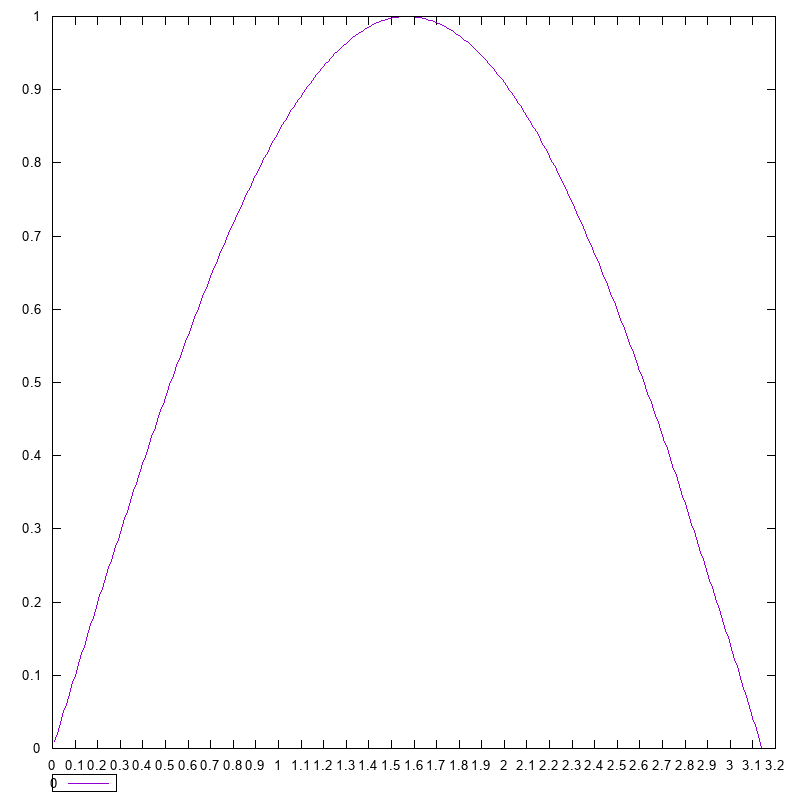
\includegraphics[scale=0.3]{../Onegraphs/Polynomial-Interpolated.png}
\caption{Polynomishe interpolant van 12de graad voor sin(x)}
\end{figure}
\begin{figure}[H]
\centering
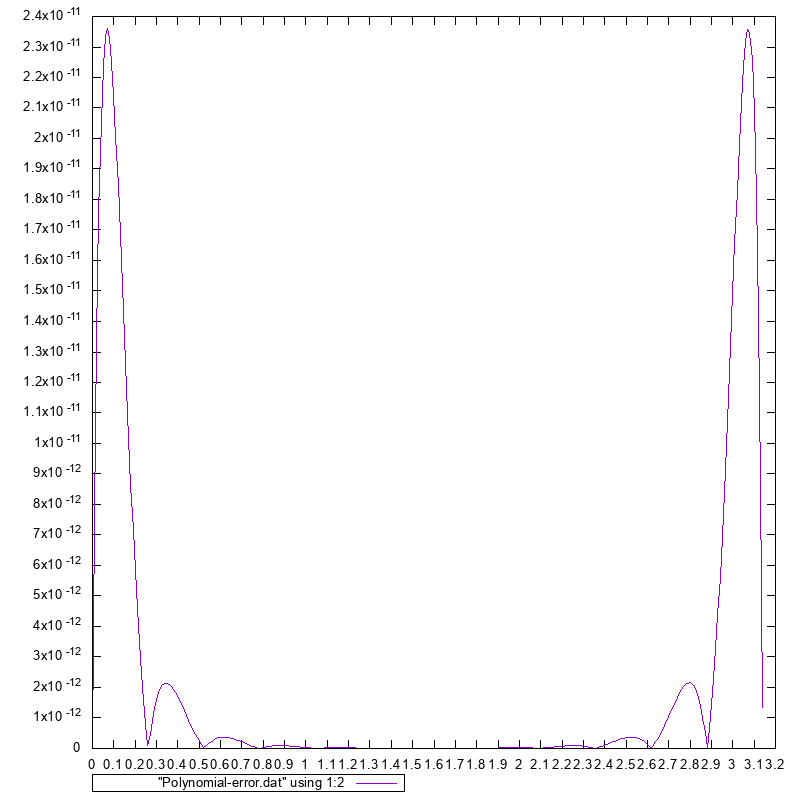
\includegraphics[scale= 0.5]{../Onegraphs/Polynomial-Error.png}
\caption{Foutenkromme voor de polynomische interpolant}
\end{figure}
Bij de foutenkromme zien we duidelijk het Runghe fenomeen optreden. Aan de buitenkanten van het interval begint de foutenkromme te oscilleren. We zullen zien bij een spline dat ze oscillatie langs de buitenkant veel kleiner is. Een andere oplossing was het verminderen van datapunten(wat niet nuttig was in dit geval gezien dat deze een hogere fout opleveren), een paar datapunten weg laten of een andere basis kiezen zoals bijvoorbeeld de chebyshev basis.
\subsection{Natuurlijke Kubische Spline}
Een andere manier om sin(x) te benaderen gaat via een natuurlijke kubische spline. We gebruiken dezelfde procedure als bij de polynomische interpolant maar gebruiken dan de GSL functies voor het tekenen van een spline die we $s(x)$ noemen. Wat opvalt is dat we deze keer geen gebruik maken van 13 datapunten maar wel 226!
\\
\\
Een natuurlijke kubische spline heeft in haar begin en eindpunt als 2de afgeleide 0. Dit is een goed idee ten eerste omdat het de berekening van een spline makkelijker maakt. We zouden een waarde kunnen geven voor de 2de afgeleide in het begin en eindpunt maar dit zou de functie meer convex of concaaf maken naar het einde toe(=de boog wordt groter).  Hieronder de geplotte spline en zijn foutenkromme.
\begin{figure}[H]
\centering
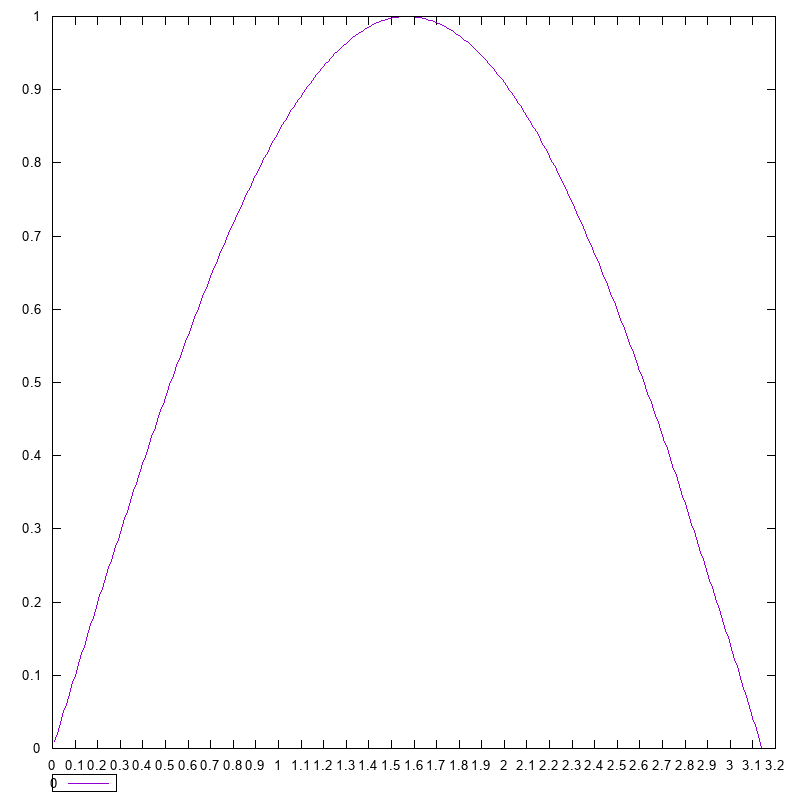
\includegraphics[scale=0.42]{../Onegraphs/Spline-Interpolated.png}
\caption{Een natuurlijke kubische spline die sin(x) benadert met 226 datapunten}
\end{figure}
\begin{figure}[H]
\centering
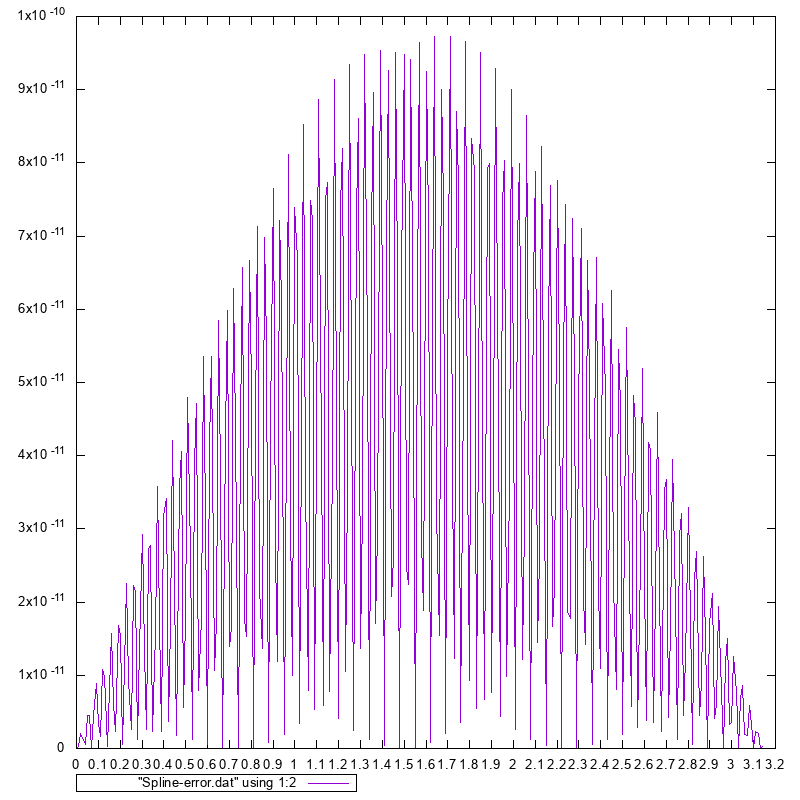
\includegraphics[scale= 0.42]{../Onegraphs/Spline-Error.png}
\caption{Foutenkromme voor de spline}
\end{figure}
We zien dat de geplotte spline de sin(x) functie mooi benadert. Wanneer we kijken naar de foutenkromme van de spline merken we veel meer oscillaties dan de polynomische interpolant maar deze zijn veel beter gedistribueerd over het interval. Dit maakt dat de fout ongeveer overal hetzelfde is t.o.v. de polynomische interpolant waarbij de fout enkel langs de uiteinden zit. Wat wel op te merken valt is dat de fout in de spline lichtjes groter is dan die van de polynomische interpolant.

\section{Opgave 2}
Berken nu met deze n + 1 datapunten van de natuurlijke kubische spline een kleinste kwadraten parabool benadering van de vorm $q(x) = a+bx+cx^{2}$ en bespreek.
\subsection{De kleinste kwadraten parabool benadering}
Door gebruik te maken van de GSL Multifit Lineair functies is het zeer simpel om een kleinste kwadraten benadering te plotten van de vorm $q(x) = a+bx+cx^{2}$. We geven volgende matrix mee waarop we de kleinste kwadraten procedure uitvoeren. De x waarden komen voort uit de gegeven n+1 datapunten. 
$$
\begin{bmatrix}
1 & x_{0} & x_{0}^{2} \\
1 & x_{1} & x_{1}^{2} \\
\vdots & \vdots & \vdots \\
1 & x_{n} & x_{n}^{2}
\end{bmatrix}
$$
Als y waarden wordt er gebruik gemaakt van volgende vector:
$$
\begin{bmatrix}
y_{0} \\
y_{1}\\
\vdots \\
y_{n}
\end{bmatrix}
$$
Dit levert dan volgend stelsel op:
$$
\begin{bmatrix}
1 & x_{0} & x_{0}^{2} \\
1 & x_{1} & x_{1}^{2} \\
\vdots & \vdots & \vdots \\
1 & x_{n} & x_{n}^{2}
\end{bmatrix}
*
\begin{bmatrix}
c_{0} \\
c_{1}\\
c_{3}
\end{bmatrix}
=
\begin{bmatrix}
y_{0} \\
y_{1}\\
\vdots \\
y_{n}
\end{bmatrix}
$$
Wanneer we GSL dit stelsen laten oplossen d.m.v. de kleinste kwadraten methode krijgen we hetvolgende polynoom:
$$
q(x) =  -0.049131235912031057111 +1.3101111168458918765x -0.41702132049133477931x^{2}
$$
Wanneer we deze functie $q(x)$ dan plotten over het interval [0, $\pi$] verkrijgen we volgende plot + tevens ook de foutenkromme $\left | f(x) - q(x)  \right |$:
\begin{figure}[H]
\centering
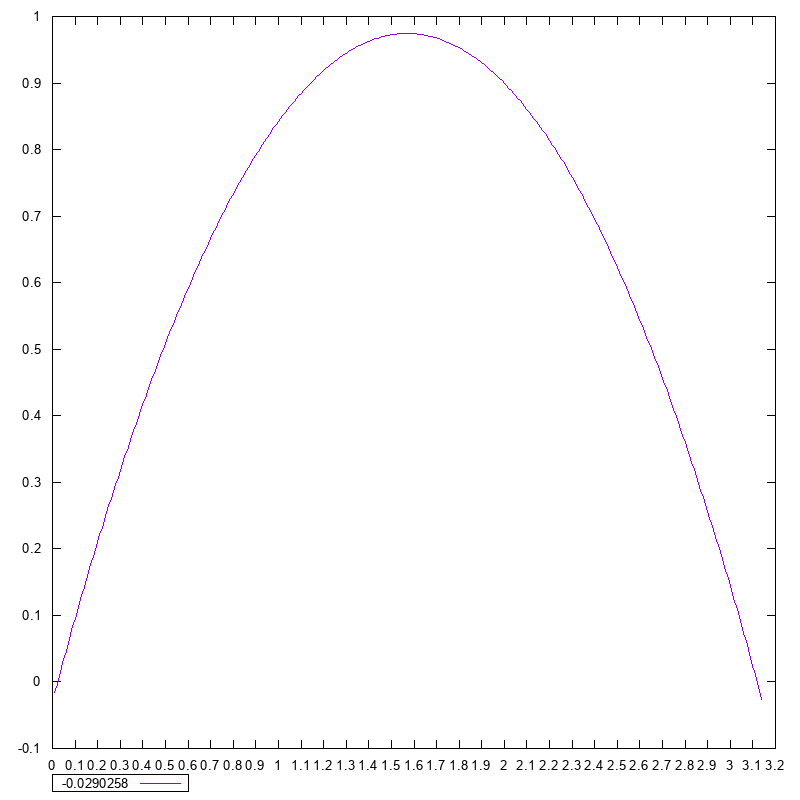
\includegraphics[scale=0.42]{../Onegraphs/LeastSquares-Interpolated.png}
\caption{Een kleinste kwadraten benadering van sin(x)}
\end{figure}
\begin{figure}[H]
\centering
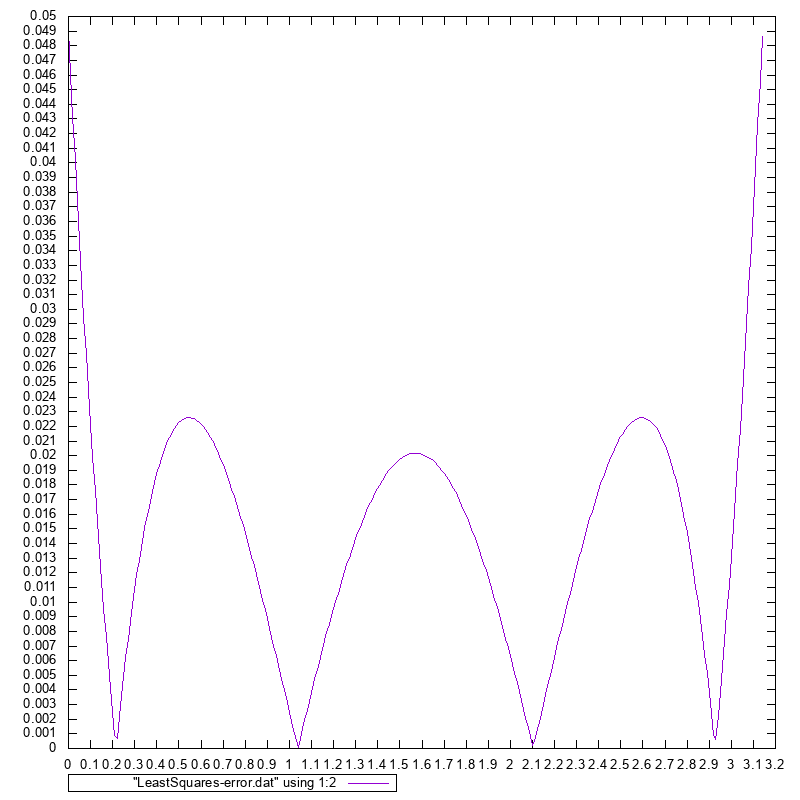
\includegraphics[scale= 0.42]{../Onegraphs/LeastSquares-Error.png}
\caption{Foutenkromme voor de kleinste kwadraten benadering}
\end{figure}
We zien dat de foutenkromme een speciale vorm heeft, met momenten is de fout nul en met andere momenten is de fout hoog. Zeer hoog zelfs de fout licht een stuk hoger dan de foout van de polynomische interpolant en de natuurlijke kubische spline. Gezien de absolute fout van de absolute waarde van de fout neemt(en er dus geen y-waarden onder 0 zijn). Kunnen we veronderstellen dat de plot van de kleinste kwadraten functie soms een positieve en soms een negatieve fout zal hebben.
\subsubsection{Vergelijkingen}
Wanneer we nu de 3 benaderingen plotten op 1 grafiek + een plot van sin(x) bekomen we volgende plot:
\begin{figure}[H]
\centering
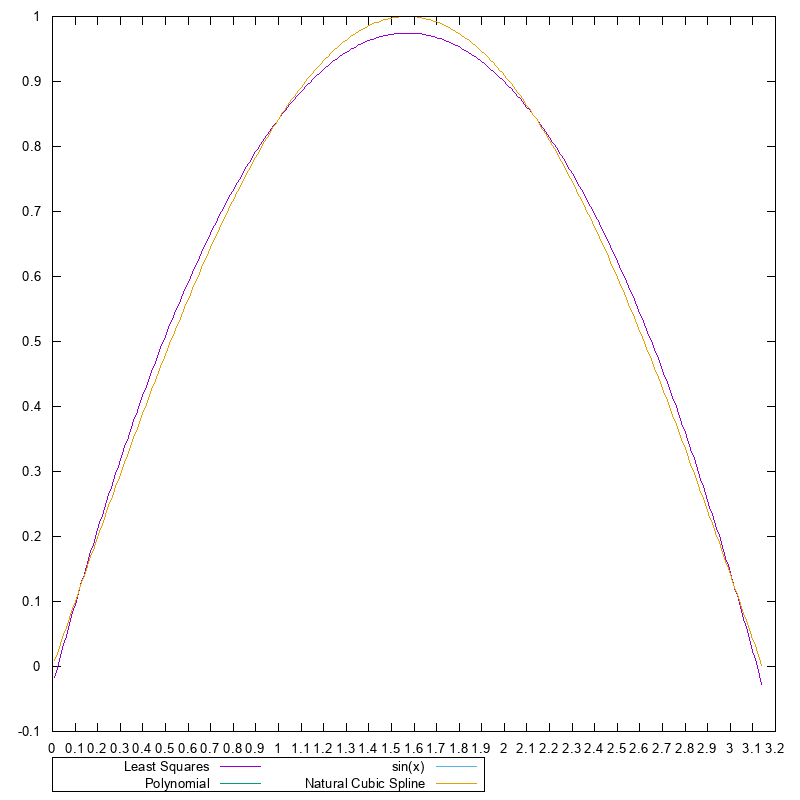
\includegraphics[scale= 0.7]{../Onegraphs/All.png}
\caption{Alle benaderingen + sin(x)}
\end{figure}
Wat opvalt is dat de polynimische interpolant, natuurlijke kubische spline en sin(x) samenvallen. Natuurlijk is dit niet zo, we hebben al eerder gezien dat de natuurlijke kubische spline haar fout anders gedistribueerd is + lichtjes groter is. Dit zijn immers kleine verschillen welke niet opvallen op de huidige grafiek, mocht men deze vergtoeten zou men duidelijker een verschil zien tussen deze 3 functies.
\\
\\
De functie die er wel uit springt is de kleinste kwadraten parabool benadering, deze loopt niet gelijk met de 3 andere en maakt zoals eerder aangehaald een zeer grote fout. Wat opvalt is dat de fout soms ook 0 is: dit zijn de punten waar de sin(x) en de kleinste kwadraten benaderin elkaar snijden. Zoals eerder aangehaald is de fout soms postitief en soms negatief. Dit zien we ook in de plot: soms light de kleinste kwadraten benadering boven de sin(x) functie en soms eronder.
\\
\\
Er is geen samenvattende plot van de foutenkrommes van de 3 benaderingen omdat deze niet duidelijk genoeg zou zijn en aan de hand van de plot van de 3 benaderingen al veel uitgelegd kan worden.
\section{Opgave 3}
Functie $f(x)$ is gelijk aan -1 op het interval [-$\pi$, 0] en +1 op het interval [0, $\pi$], bereken enkele benaderingen. Maak gebruik van $n \geq 120$ equidistante punten.
\subsection{Veelterm Interpolanten}
Er werd gevraagd om enkele veelterm interpolanten te berekenen. Om te bepalen welke graad te gebruiken berekenen we telkens de relative fout : 
$$ \left | \frac{x_{berekend} - x}{x}  \right |$$
Uiteindelijk kiezen we 2 manieren voor het selecteren van punten(zie opgave 1, hoe meer punten geselecteerd, hoe harder het runghe fenomeen kan optreden).
\\
\\ 
Ten eerste selecteren we punten op een equidistante afstand van elkaar, we laten deze afstand steeds kleiner worden en dus in het begin worden niet alle punten gebruikt. Wanneer we deze procedure uitvoeren op 241 punten valt op dat de relatieve fout het kleinst is wanneer we een polynomische interpolant van graad 240 construeren met 241 datapunten. Dit levert relatieve fout op van : 4.2881891672892731293 . 
\begin{figure}[H]
\centering
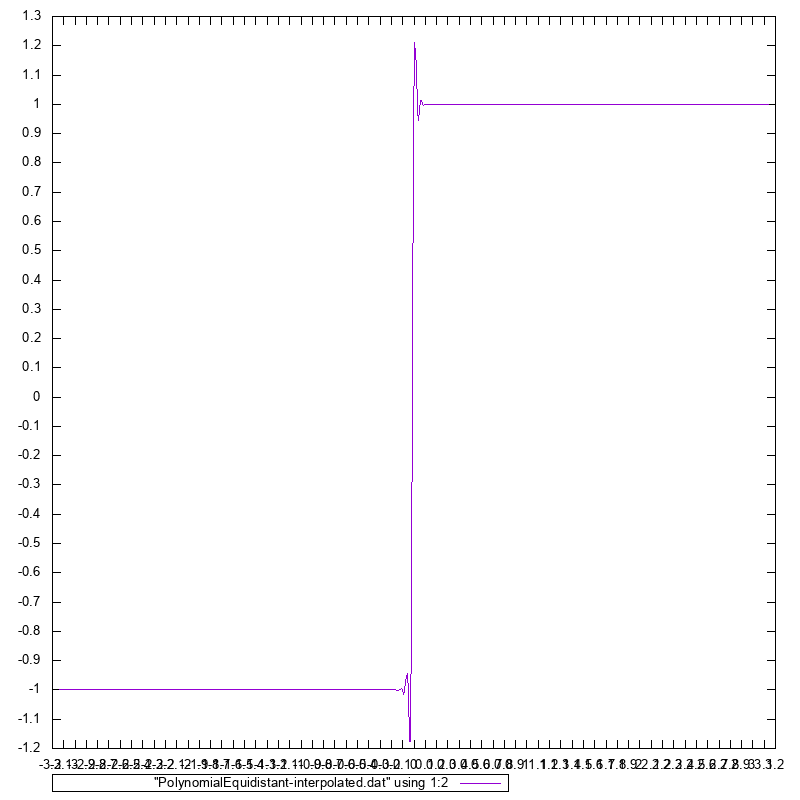
\includegraphics[scale=0.3]{../Twographs/PolynomialEquidistant-interpolated}
\caption{Een polynomische equidistante interpolant van f(x) van graad 240}
\end{figure}
\begin{figure}[H]
\end{figure}
De interpolant benadert de functie vrij goed behalve rond de x-waarde 0.
\\
\\
Een andere manier van punten selecteren is door deze niet equidistant te kiezen maar random over het interval te selecteren. Wanneer we deze procedure toepassen verkijgen we een polynoom van de graad 183 met 182 datapunten waarbij de relative fout 2.5545165758846741788 is. We zien dit ook op de plot van de interpolant:
\begin{figure}[H]
\centering
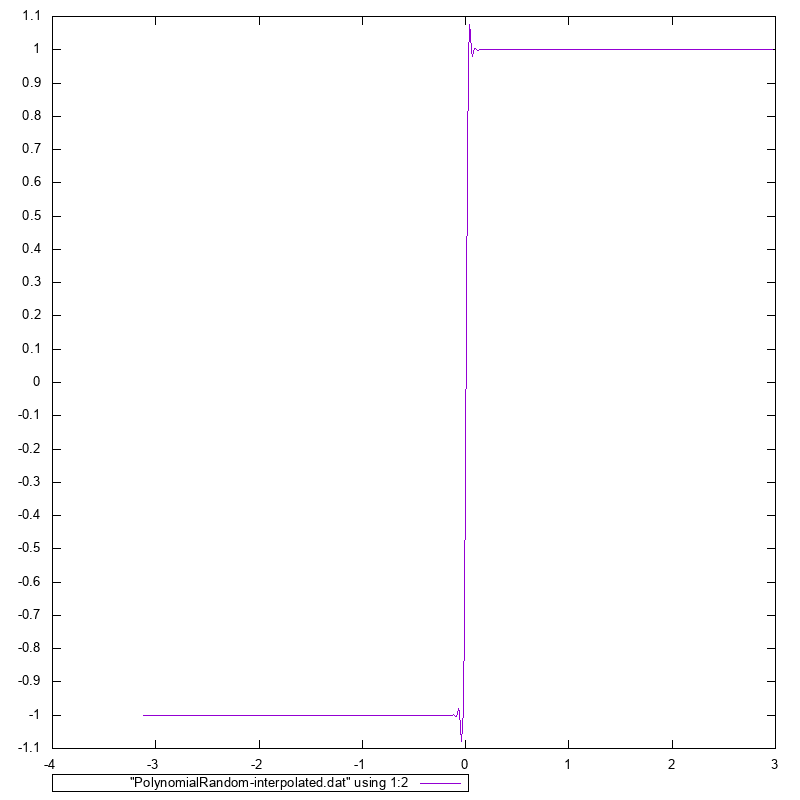
\includegraphics[scale=0.3]{../Twographs/PolynomialRandom-interpolated}
\caption{Een polynomische random interpolant van f(x) van graad 240}
\end{figure}
\begin{figure}[H]
\end{figure}
Waarbij de equidistante punten de y-waarden rond 0 nog tot ongeveer 1.3 lopen door osccilaties, lopen ze bij random gekozen punten maar tot 1.1 een duidelijk verschil! Daarom kiezen we dus voor een polynomishce interpolant met random gekozen punten inplaats van equidistante punten.
\subsection{Kleinste kwadraten veeltermbenadering}
TODO
\subsection{Trigonometrische veelterminterpolant}
Voor de trigoniometrische veelterminterpolant berekenen we enkele coefficienten met $i = 1 \hdots m$:
$$
a_{i} = \frac{2}{n}\sum^{n - 1}_{k = 0}(y_{k}*cos(i * x_{k})) 
$$
$$
b_{i} = \frac{2}{n}\sum^{n - 1}_{k = 0}(y_{k}*sin(i * x_{k})) 
$$
Bij trigonometrische veelterminterpolatie stellen we dat n = 2*m dus in dit geval kiezen we voor n = 122 en m = 61. Hierdoor verkrijgen we een interpolant met als relatieve fout : 19.13715151604820619. Welke tamelijk groot is t.o.v. de polynomische interpolant. Hieronder een plot:
\begin{figure}[H]
\centering
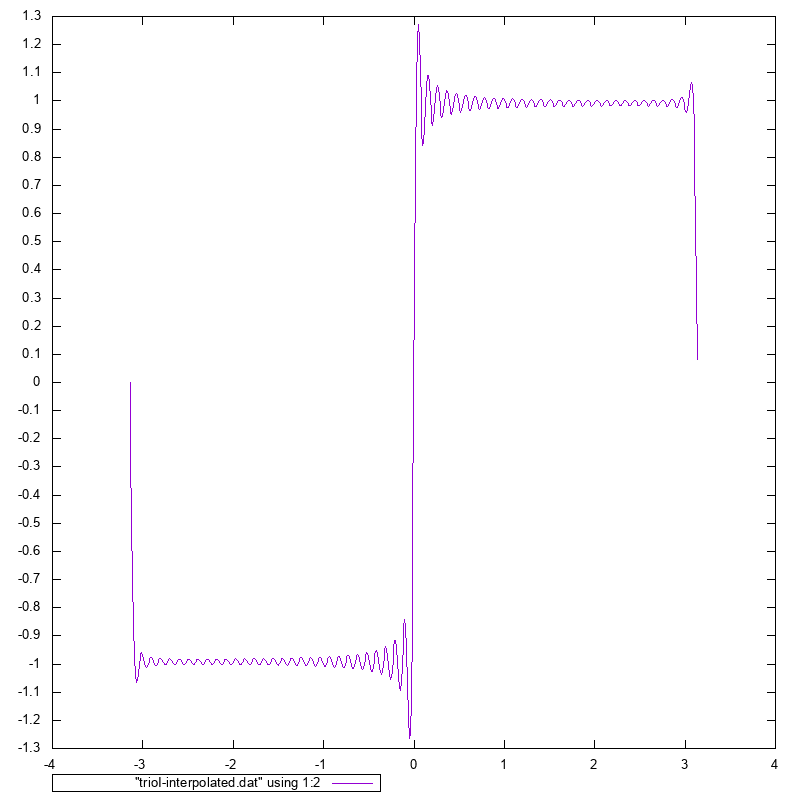
\includegraphics[scale=0.3]{../Twographs/trioI-interpolated}
\caption{Een trigonometrische veelterminterpolant van f(x)}
\end{figure}
\begin{figure}[H]
\end{figure}
Om de plot te te tekenen wordt gebruik gemaakt van volgende functie : 
$$
p(x) = \frac{a_{0}}{2} + \sum_{i = 1}^{m}(a_{i} * cos(i * x)) + \sum_{i = 1}^{m}(b_{i} * sin(i * x))
$$ 
Wat handig is dat de opgave bestaat uit equidistante punten : TODO
\subsection{Trigonometrische kleinste-kwadraten approximant}
Hierbij stellen we dat $n \geq 2*m$ en dus hebben we gekozen voor n = 121 en m = 25. We kiezen hierbij voor een oneven aantal termen(25) hierbij worden de coefficienten $a_{i} en b_{i}$ niet meer berekend van $i = 1 \hdots m$ maar van $i = 1 \hdots m-1$. Tevens komt er een extra factor bij : $\frac{1}{2}*a_{m}*cos(m * x)$. Dit levert volgende functie op:
$$
p(x) = \frac{a_{0}}{2} + \sum_{i = 1}^{m-1}(a_{i} * cos(i * x)) + \sum_{i = 1}^{m-1}(b_{i} * sin(i * x)) + \frac{1}{2}*a_{m}*cos(m * x)
$$
Dit verschil tussen een oneven/even aantal termen zorgt ervoor dat : TODO
\\
\\
De relative fout van deze benadering is : 34.455640624730698107. Wanneer we de functie $p(x)$ plotten krijgen we volgende functie : 
\begin{figure}[H]
\centering
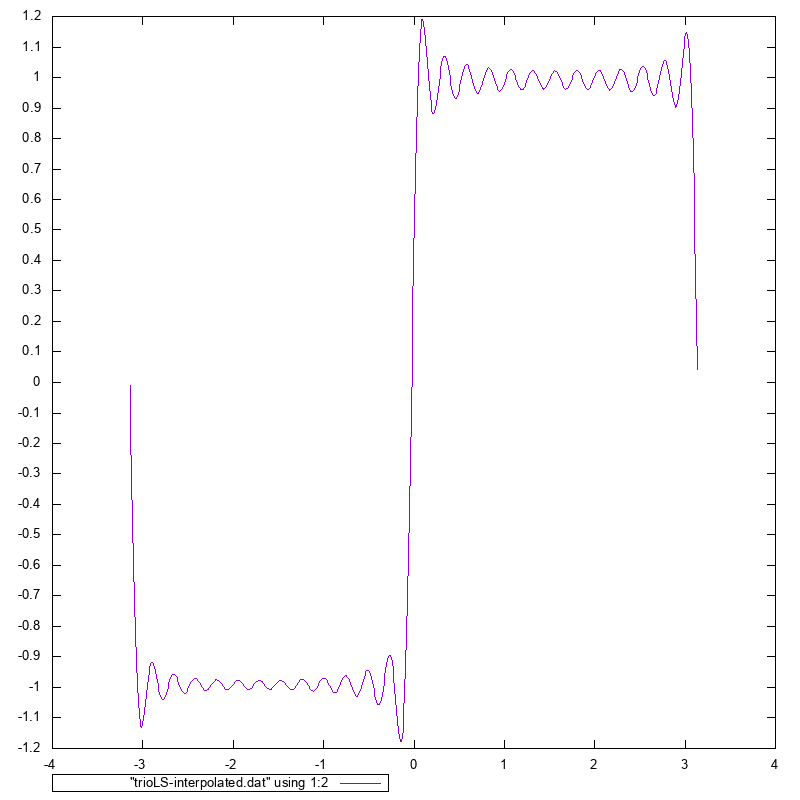
\includegraphics[scale=0.3]{../Twographs/trioLS-interpolated}
\caption{Trigonometrische kleinste-kwadraten approximant van f(x)}
\end{figure}
\begin{figure}[H]
\end{figure}
\subsection{Vergelijken}
\begin{figure}[H]
\centering
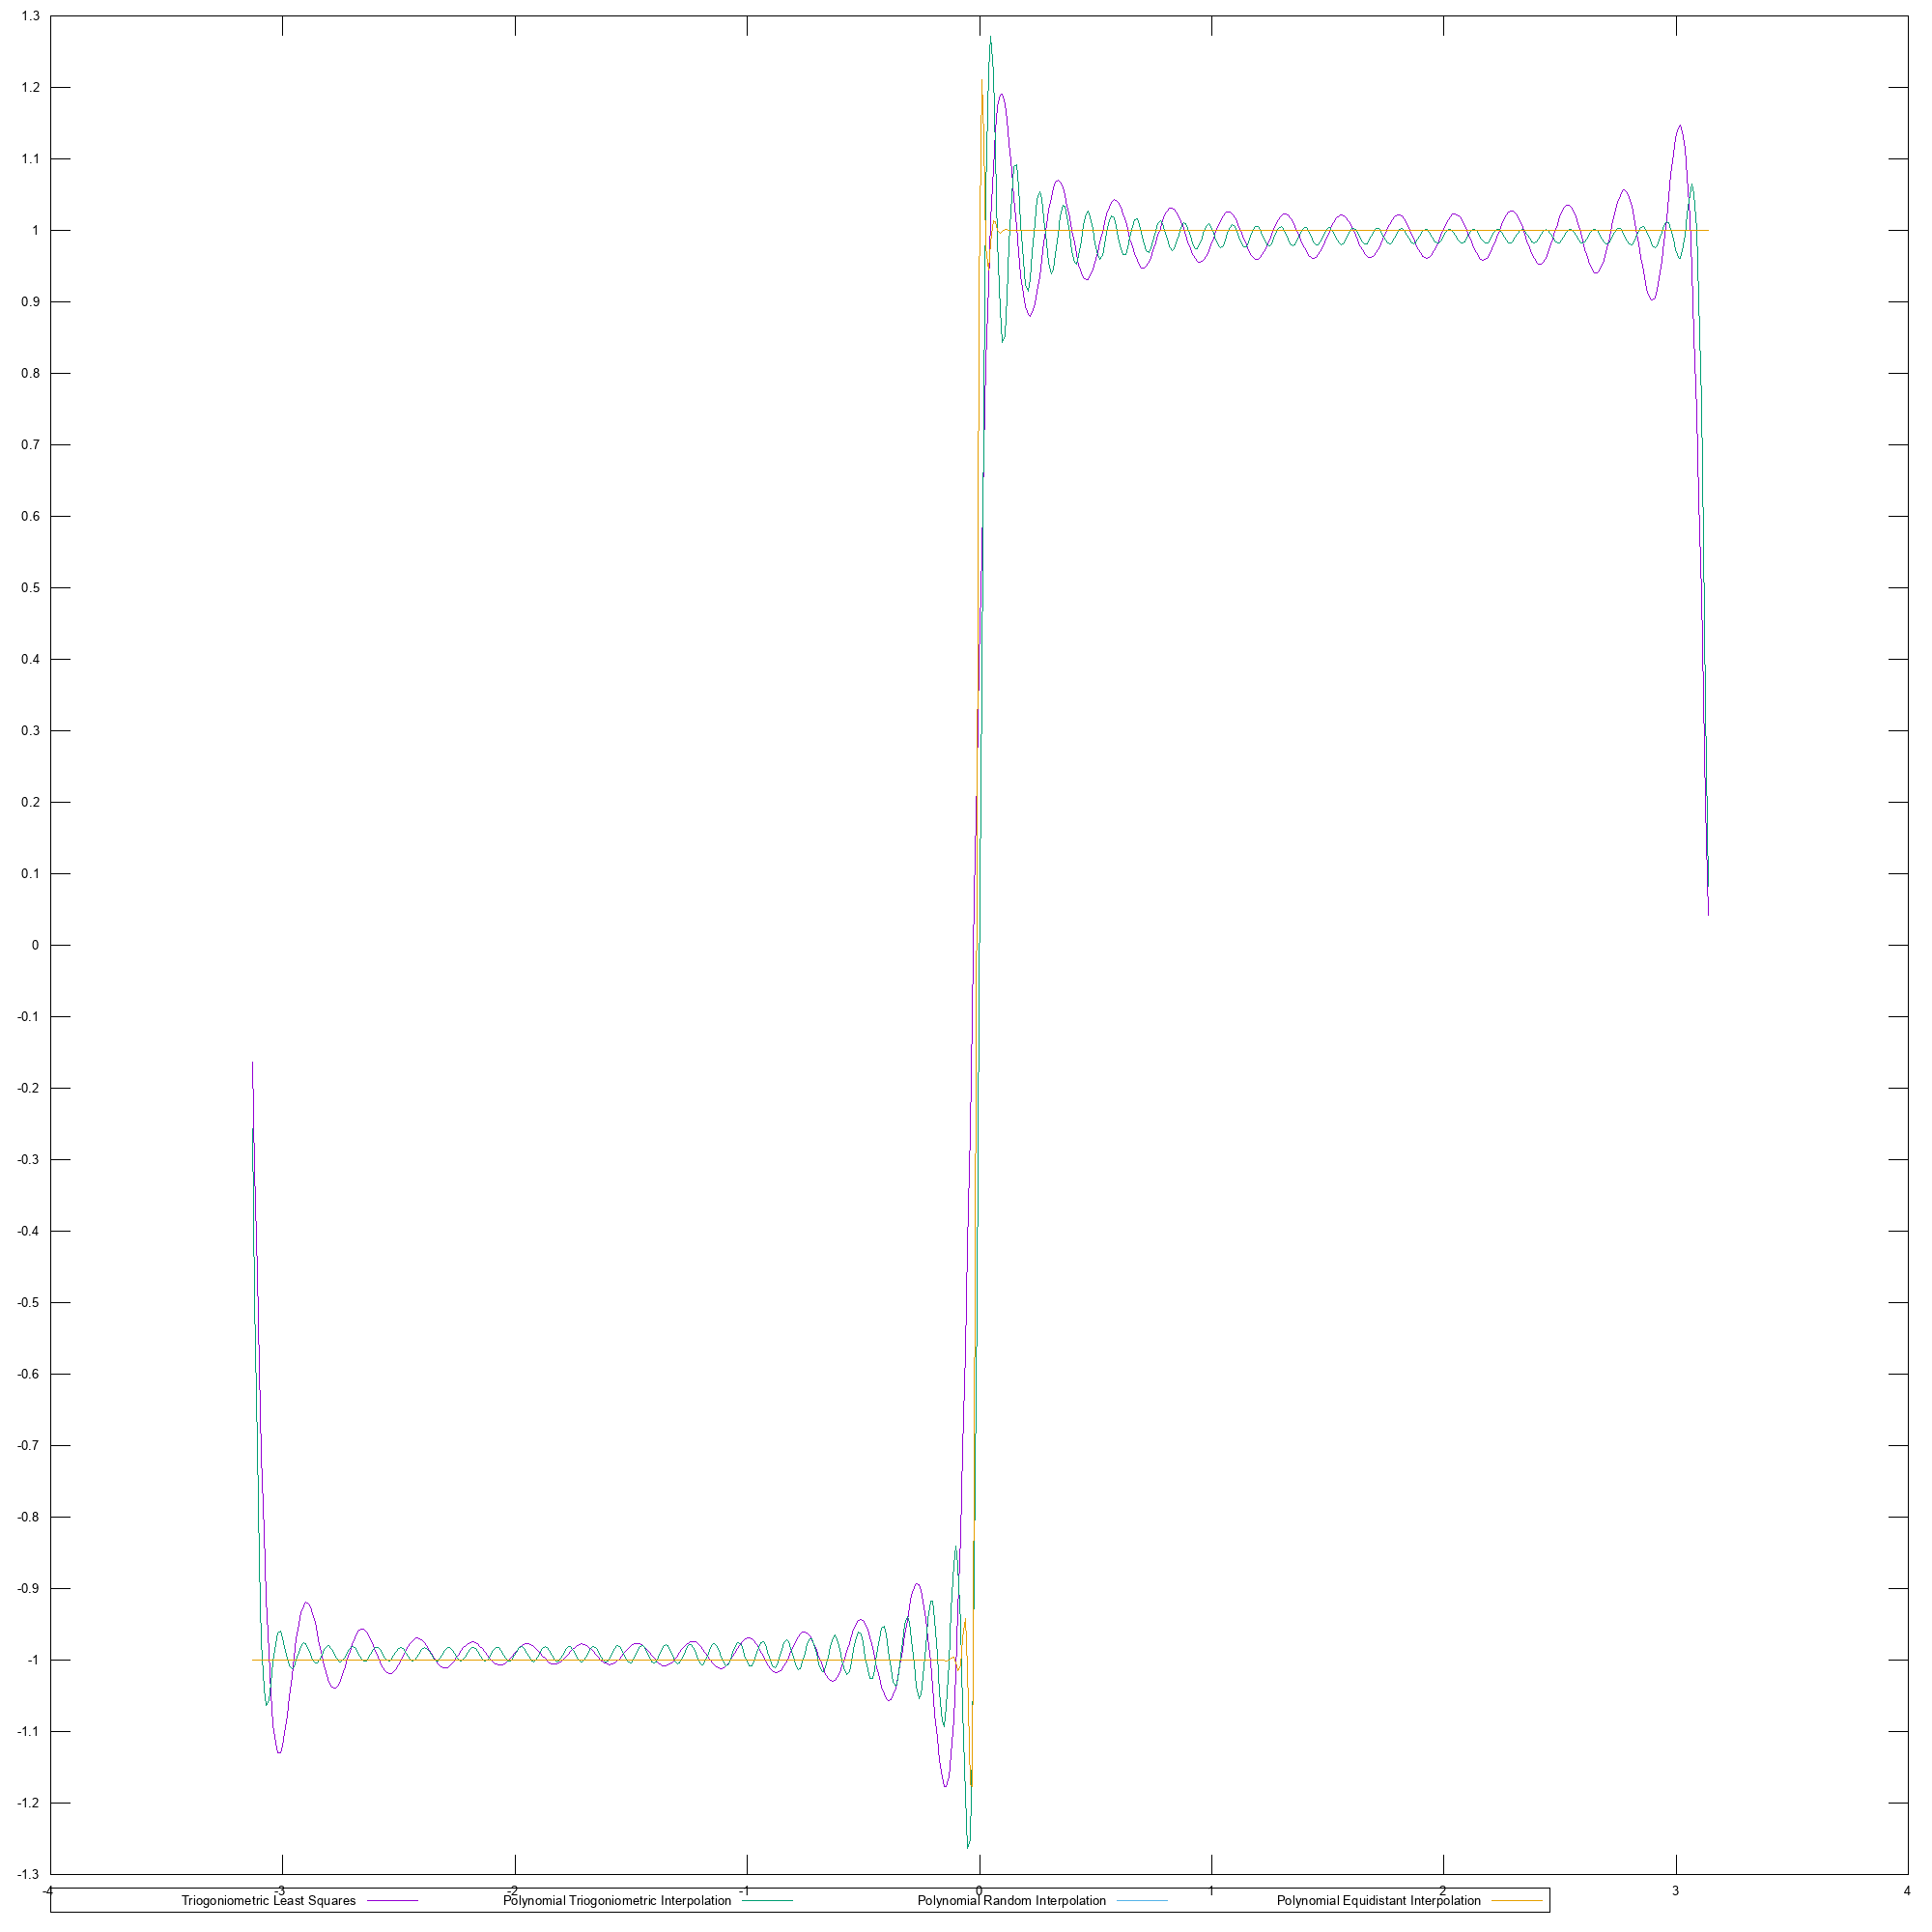
\includegraphics[scale=0.3]{../Twographs/All}
\caption{Alle benaderingen van opgave 4}
\end{figure}
\begin{figure}[H]
\end{figure}
Wanneer we nu alle benaderingen naast elkaar zetten op een afbeelding zien we dat de Polynomische Interpolant met random gekozen punten f(x) het beste benadert, gevolgd door de Polynomische interpolant met equidistante punten. Daarna de trigonometrische interpolant en vervolgens de Trigonometrische kleinste-kwadraten approximant. Dit zagen we ook eerder in de fouten die de beanderingen hadden.
\section{Opgave 4}
Gebruik de n+1 datapunten die de polynomische interpolant p(x) in opgave 1 opleverde en stel een stelsel interpolatievoorwaarden op, bereken het conditiegetal en los het op met GEPP.
Het stelsel zal volgende vorm hebben:
$$
\begin{bmatrix}
1 & x_{0} & x_{0}^{2} & \hdots x_{0}^{n}  \\
1 & x_{1} & x_{1}^{2} & \hdots x_{1}^{n}\\
\vdots & \vdots & \vdots & \vdots \\
1 & x_{n} & x_{n}^{2} & \hdots x_{n}^{n}
\end{bmatrix}
*
\begin{bmatrix}
c_{0} \\
c_{1}\\
\vdots \\
c_{n}
\end{bmatrix}
=
\begin{bmatrix}
y_{0} \\
y_{1}\\
\vdots \\
y_{n}
\end{bmatrix}
$$
Hierbij zijn de x en y waarden al gekend uit de n + 1 datapunten uit opgave 1. Dit levert het volgende stelsel op:
\\
\\
\resizebox{\textwidth}{!}{%
$A=\begin{bmatrix}
1 & 0 & 0 & 0 & 0 & 0 & 0 & 0 & 0 & 0 & 0 & 0 & 0 \\
1 & 3.1 & 9.9 & 31 & 97 & 3.1e+02 & 9.6e+02 & 3e+03 & 9.5e+03 & 3e+04 & 9.4e+04 & 2.9e+05 & 9.2e+05 \\
1 & 0.5 & -2.5 & -12 & -43 & -1.4e+02 & -4.7e+02 & -1.5e+03 & -4.7e+03 & -1.5e+04 & -4.7e+04 & -1.5e+05 & -4.6e+05 \\
1 & 0.75 & 0.75 & -1.5 & -10 & -49 & -2e+02 & -7.5e+02 & -2.6e+03 & -9e+03 & -3e+04 & -9.8e+04 & -3.2e+05 \\
1 & 0.17 & 0.56 & -0.99 & -2.6 & -20 & -1e+02 & -4.2e+02 & -1.6e+03 & -5.6e+03 & -1.9e+04 & -6.4e+04 & -2.1e+05 \\
1 & 0.92 & 0.31 & 0.68 & 0.2 & -1.2 & -13 & -83 & -4.3e+02 & -2e+03 & -8.3e+03 & -3.3e+04 & -1.2e+05 \\
1 & 0.33 & 0.89 & -0.79 & 0.57 & 0.65 & 1.4 & 17 & 1.2e+02 & 6.3e+02 & 3e+03 & 1.3e+04 & 5.2e+04 \\
1 & 0.083 & 0.31 & -0.68 & 0.79 & -0.44 & -0.98 & 1.1 & 13 & 93 & 5.1e+02 & 2.4e+03 & 1.1e+04 \\
1 & 0.83 & 0.56 & 0.99 & 0.14 & 0.65 & 0.14 & 0.29 & 0.76 & 11 & 92 & 5.9e+02 & 3.2e+03 \\
1 & 0.58 & 0.97 & 0.43 & -0.12 & -0.35 & -0.31 & -0.32 & -0.73 & 0.44 & 7.1 & 66 & 4.6e+02 \\
1 & 0.25 & 0.75 & -1 & 0.87 & 0.49 & 0.87 & -0.29 & -0.23 & 0.72 & -0.33 & -5.6 & -54 \\
1 & 0.67 & 0.89 & 0.79 & -0.11 & -0.39 & -0.26 & -0.35 & -0.93 & 0.85 & -0.3 & 0.13 & 2.4 \\
1 & 0.42 & 0.97 & -0.43 & 0.25 & 0.42 & 0.56 & 0.19 & 0.29 & -0.67 & -0.46 & 0.63 & -0.063
\end{bmatrix}$%
}
\\
\\
Dit levert volgend stelsel op : 
$$
A * \begin{bmatrix}
c_{0} \\
c_{1}\\
\vdots \\
c_{n}
\end{bmatrix} 
= 
\begin{bmatrix}
0 \\
0.25881904510252073948 \\
0.49999999999999994449 \\
0.70710678118654746172 \\
0.86602540378443859659 \\
0.96592582628906820119 \\
1 \\
0.96592582628906831221 \\
0.86602540378443881863 \\
0.70710678118654757274 \\
0.50000000000000033307 \\
0.25881904510252101703 \\
1.2246467991473532072e-16
\end{bmatrix}
$$
Vervolgens berekenen we het conditiegetal van de matrix A om vervolgens te kijken naar de orde van de relatieve fout van de oplossing. Het berekenen van het conditiegetal gebeurt d.m.v. een singuliere waarden decompositie(GSL Linalg SV Decomp) waarbij de minimale en maximale singuliere waarde wordt gezocht en deze door elkaar worden gedeeld. Wanneer dit wordt uitgevoerd komen we op volgende:
$$
\kappa (A) = 418891964854.25164795 \approx 4*10^{12}
$$
GEPP is niet stabiel:
$$
\left \| \tilde{x} - x^{\star}) \right \| \leq n^3*ULP*\kappa(A)*\left \|  x^{\star} \right \|
$$
Hieruit halen we dat de onvermijdelijke relative afrondingsfout  $n^{3}*ULP$ wordt opgeblazen op $x^{\star}$ (de exacte oplossing) met een factor $\kappa(A)$, het conditiegetal. Dit grote conditiegetal zorgt ervoor dat de fout wordt vergroot met een factor $10^{12}$. Op mijn computer was ULP = $2.2*10^{-16}$ en $n^3 = 2197 = 2 * 10^{2}$. Dit zorgt ervoor dat de fout van GEPP ongeveer gelijk is aan: 
$$  10^{2} * 0^{12} * 10^{-16} = 10^{-2} = 0.01$$
Dit is een zeer hoge fout en er kan dus verwacht worden dat resultaten niet altijd even correct zijn.
\\
\\
Als laatste nog de uitkomstenvector van de GEPP procedure, hiermee kan vervolgens een interpolatiepolynoom $p(x) = c_{0} + c_{1}x + c_{2}x^{2} + \hdots + c_{n}x^{n}$ worden opgesteld om zo de sin(x) functie benaderen.
\\
$$
C =  \begin{bmatrix}
0 \\
0.99999999913751358438 \\
1.0761642333038017988e-08 \\
-0.16666672378000291221 \\
1.7343027474583990613e-07 \\
0.0083329935383840807173 \\
4.570069542541168747e-07 \\
-0.00019884908285970522837 \\
3.0059277657056513061e-07 \\
2.6061122447290966013e-06 \\
5.309884908907600906e-08 \\
-3.8025144634222871813e-08 \\
2.0172966316920489529e-09 \\
\end{bmatrix} 
$$
\subsection{Opgave 5}
Bereken het volume van een cylinder met als grondvlak $\Omega  = (x-0.5)^{2} + (y-0.5)^{2} \leq 0.25 $ en als hoogte $ln(x + y)$ tot 2 beduidende cijfers correct.
\subsubsection{MAPLE}
Om te kunnen weten of de berekende oplossing tot 2 beduidende cijfers correct is wordt gebruik gemaakt van MAPLE om een exacte oplossing voor het volume van de cylinder te vinden. Dit kan d.m.v. volgende code:
\begin{lstlisting}
with(VectorCalculus);
int(abs(ln(x+y)), [x, y] = Circle({0.5,0.5}, .5));
\end{lstlisting}
Wanneer we dit uitrekenen bekomen we dat het volume $I = 0.2550197403$.
\subsubsection{Berekening}
Om het volume te bereken maken we gebruik van Monte Carlo Integratie deze gebruikt random samples en kijkt of deze (x, y) coordinaten in het volume liggen of niet. Om deze conditie te checken geven we volgende functie aan GSL mee :
\begin{lstlisting}
double func (double x[], size_t dim, void * p){
    if (dim != 2)
    {
        fprintf (stderr, "error: dim != 2");
        abort ();
    }

    if(pow(x[0] - 0.5, 2) + pow(x[1] - 0.5, 2) <= 0.25){
        return fabs(log(x[0] + x[1]));
    }else{
        return 0.0;
    }
}
\end{lstlisting}
Indien het(x,y) coordinaat in het grondvlak ligt, zal het een hoogte mee krijgen bepaald door$ln(x+y)$ ligt het niet in het grondvlak, dan krijgt het de hoogte 0 mee. Wanneer we dit uitrekenen en met een seed = 123 en random generator = mrg. Is met 691 samples de inhoud gelijk aan 0.25936620629454121278 wat de gelijkenis van 0.25 heeft met de MAPLE berekening.
\section{Code}
\textbf{../one.cpp - Opgave 1, 2 en 4}
\lstinputlisting{../one.cpp}

\textbf{../one.cpp - Opgave 3}
\lstinputlisting{../two.cpp}

\textbf{../three.cpp - Opgave 5}
\lstinputlisting{../three.cpp}

\end{document}